\chapter{Simpliziale Mengen}
\section{Triangulierte Räume}
\subsection{Definitionen}

\begin{definition}
  Ein \emph{Triangulierter Raum} besteht aus
  \begin{itemize}
    \item Punkten,
    \item Kanten,
    \item Dreiecke,
    \item Tetraeder,
    \item \ldots
    \item $n$-dimensionale Simplizes
  \end{itemize}
  und einer kombinatorischen Verklebevorschrift.
\end{definition}

\begin{definition}[topologischer $n$-Simplex, Ecke, $I$-Fläche]
  Der \emph{$n$-dimensionale topologische Simplex} (oder \emph{topologischer
  $n$-Simplex}) ist der topologische Raum
  \[ \Delta_n \speq{:=} \big\{(x_0,\ldots,x_n) \in \R^{n+1} \mid 
    \sum_{i=0}^n x_i = 1,\ x_i \geq 0\big\}\,.\]
  Der Punkt $e_i \in \Delta_n$ mit $x_i=1$ heißt die \emph{$i$-te Ecke von
  $\Delta_n$}.\\
  Für $I \subseteq [n] := \{0,\ldots,n\}$ ist die \emph{$I$-Fläche von
  $\Delta_n$} durch
  \[ \big\{(x_0,\ldots, x_n) \in \Delta_n \mid 
    x_i = 0 \ \forall i\notin I\big\}\]
  gegeben.
\end{definition}

\begin{bemerkung}
  Durch obige Definition einer Ecke erhält man eine Anordnung der Ecken!
\end{bemerkung}

\begin{beispiel}[Veranschaulichung verschiedener topologischer $n$-Simplizes]
  \begin{description}
    \item[$n=0$] \Bild
    \item[$n=1$] \Bild
    \item[$n=2$] \Bild
  \end{description}
\end{beispiel}


\begin{bemerkung}
  Jedes $I\subseteq [n]$ mit $|I| = m+1$ definiert genau eine streng monoton
  wachsende Abbildung 
  $f: [m]  \to  [n]$ mit $\im f = I$.
  Diese Konstruktion ist umkehrbar.
\end{bemerkung}

\begin{definition}
  Die Abbildung 
  \[ \Delta_f:\ \Delta_m \to \Delta_n\]
  ist diejenige lineare Abbildung, welche die Ordnung der Ecken berücksichtigt
  und die $I$-Seite von $\Delta_n$ als Bild hat, wobei $f$ und $I$ nach obiger
  Bemerkung korrespondieren.
\end{definition}

\begin{beispiel}
  Für 
  \[ f: \funcdef{[1]& \to &[2] \\ 0 &\mapsto& 0\\ 1&\mapsto&2}
    \quad\leftrightarrow\quad I = \{0,2\}\]
  erhalten wir $\Delta_f:\ \Delta_1\to\Delta_2$: \Bild
\end{beispiel}


\begin{definition}
  Ein \emph{Verklebedatum $X$} ist eine Folge 
  $X_{(0)}, X_{(1)}, \ldots$ von Mengen,
  wobei man $X_{(0)}$ als \emph{Punkte}, $X_{(1)}$ als \emph{Kanten}, 
  $X_{(2)}$ als \emph{Flächen}, \ldots bezeichnet und für jede streng 
  monotone Abbildung $f:\ [m]\to[n]$ eine Abbildung
  \[ X(f):\ X_{(n)} \to X_{(m)}\,,\]
  so dass Folgendes gilt:
  \begin{enumerate}
    \item $X(\id_{[n]}) = \id_{X_{(n)}}$,
    \item $X(g\circ f) = X(f)\circ X(g)$.
  \end{enumerate}
\end{definition}

\begin{beispiel}
  \label{bsp:2-simplex-x}
  Für $\Delta_2$ haben wir:
  \begin{center}
    \begin{minipage}{0.4\textwidth}
      \Bild
      \centering
      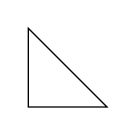
\begin{tikzpicture}
        \path[draw] (0,0) -- (0,1) -- (1,0) --cycle;
      \end{tikzpicture}
    \end{minipage}
    \hfill
    \begin{minipage}{0.4\textwidth}
      \begin{align*}
        X_{(0)} \speq{:=} \{ \Bild\}\\
        X_{(1)} \speq{:=} \{ \Bild\}\\
        X_{(2)} \speq{:=} \{ \Bild\}
        \end{align*}
      Alle weiteren $X_{(3)} = X_{(4)} = \emptyset$ sind leer.
    \end{minipage}
  \end{center}
\end{beispiel}

\begin{definition}[topologische Realisierung]
  \label{def:top-realisierung}
  Die \emph{topologische Realisierung |X| von $X$} ist der topologische Raum,
  dessen zugrunde liegende Menge durch 
  \[ \Big(\coprod_{n=0}^\infty (\Delta_n \times X_{(n)})\Big)\ \big/ \ R\]
  gegeben ist, wobei $R$ die schwächste Äquivalenzrelation ist, für die
  \[ (s,x)\ R\ (t,y) \quad\Leftarrow\quad \left\{
    \begin{array}{l}
    y = X(f)(x) \text{ und} \\ 
    s = \Delta_f(t) \text{ für ein }f:[m]\to [n]\,.
    \end{array}\right.\] 
  Für $(s,x) R (t,y)$ schreibe auch $(s,x) \overset{f}{\mapsto} (t,y)$.
  Die Topologie von $|X|$ ist die feinste Topologie, so dass
  \[ \coprod_{n=0}^\infty (\Delta_n \times X_{(n)})\ \xrightarrow{\tau}\ 
    \left(\coprod_{n=0}^\infty (\Delta_n \times X_{(n)}) \right)\big/ R = X\]
  stetig ist, d.h. $\U \subseteq |X|$ offen $\Leftrightarrow$ 
  $\tau\inv(\U)$ offen $\Leftrightarrow$ $\tau\inv(\U)$ in allen $\Delta_n$
  offen.
\end{definition}


\begin{bemerkung}
  Die definierende Gleichung der Relation $R$ in 
  \thref{def:top-realisierung} definiert zwar eine reflexive und transitive
  Relation, jedoch keine symmetrische!
\end{bemerkung}

\subsection{Beispiele}

\begin{beispiel}[$n$-dimensionaler Simplex]
  \begin{align*}
    X_{(i)} \speq{&=} \{ I\subseteq [n] \mid |I| = i+1\}\\
    \speq{&\cong} \{ f: [i] \to [n] \text{ streng monoton}\}
  \end{align*}
  \[ X([i] \xrightarrow{f} [j]):\ 
    (g:[j]\to[n]) \ \longmapsto\  (g\circ f: [i]\to[n])\,.\]
  Damit ist der $n$-dimensionale Simplex also nichts anderes, als die
  geometrische Realisierung von obigem Verklebedatum: $\Delta_n \approx |X|$.
\end{beispiel}

\begin{beispiel}[$n$-dimensionale Sphäre]
  Die Einheitsspähre $S^n$ lässt sich durch $\dell\Delta_n$ triangulieren und
  erhält damit als Verklebedatum:
  \[ X_{(i)} \speq{:=} \begin{cases}
    X_{(i)}^{\Delta_n} = \{[i] \to [n] \text{ streng monoton wachsend}\}
      & i < n\,,\\
      \emptyset & i \geq n\,,\end{cases}\]
  wobei $X^{\Delta_n}$ das Verklebedatum des $n$-Simplex meint.
  Damit erhalten wir wiederum $S^n \approx |X|$.
\end{beispiel}
